\documentclass{article}
\usepackage[utf8]{inputenc}
\usepackage{graphicx}
\usepackage{amsmath}
\usepackage[fleqn]{mathtools}
\title{Double Pendule}
\author{halebanc}
\date{}
\begin{document}

\maketitle

Nous allons montrer comment obtenir les équations différentielles du double pendule.
Voici schéma d'un double pendule avec les angles $\alpha$ et $\beta$, les longueurs $l_1$ et $l_2$ et avec deux point de jonctions chacun de masse$m_1$ et $m_2$.
\begin{figure}[!ht]
    \center
    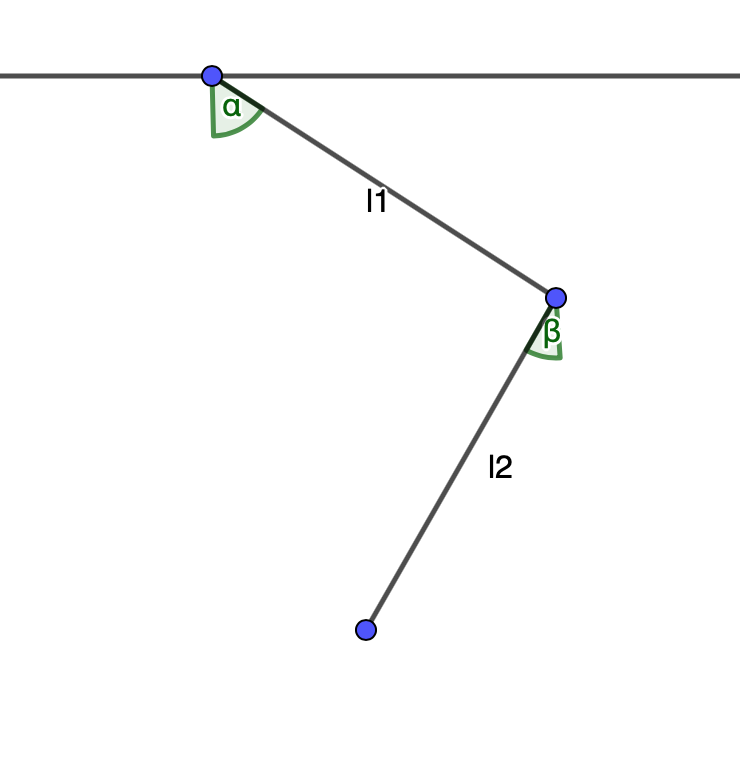
\includegraphics[scale=0.5]{double_pendule.png}
\end{figure}

Nous utiliserons le formalisme Lagrangien via les équations de Euleur-Lagrange pour obtenir les équations différentielle. 

Commençons par exprimer $x_1$, $y_1$ et $x_2$, $y_2$ et leurs dérivés en fonction des coordonnés du problèmes.

\begin{align*}
    x_1=l_1 sin(\alpha) \quad \quad
    \dot{x}_1=l_1 \dot{\alpha} cos(\alpha)
    \\
    y_1=-l_1 cos(\alpha) \quad \quad
    \dot{y}_1=l_1 \dot{\alpha} sin(\alpha)
\end{align*}

\begin{align*}
    x_2=x_2+l_2 sin(\beta)= l_1 sin(\alpha)+l_2 sin(\beta)\quad \quad
    \dot{x}_2=l_1 \dot{\alpha} cos(\alpha)+l_2 \dot{\beta} cos(\beta)
    \\
    y_2=y1-l_2 cos(\beta)=-l_1 cos(\alpha)-l_2 cos(\beta) \quad \quad
    \dot{y}_2=-l_1 \dot{\alpha} sin(\alpha)-l_2 \dot{\beta} sin(\beta)
\end{align*}

Le Lagrangien s'exprime dans notre cas comme:
$$
L=T-V 
$$
Où $L$ est l'énergie cinétique est $V$ l'énergie potentielle. 
\\Calculons dans un premier temps l'énergie cinétique $T$:
\begin{gather*}
    T=\frac{1}{2}m v^2=\frac{1}{2}m v_1^2+\frac{1}{2}m v_2^2
    =\frac{m_1}{2}(\dot{x_1}^2+\dot{y_1}^2)+\frac{m_2}{2} (\dot{x_2}^2+\dot{y_2}^2) \\
    =\frac{m_1}{2}(l_1^2 \dot{\alpha}^2 cos^2(\alpha)+l_1^2\dot{\alpha}^2 sin^2(\alpha))+\frac{m_2}{2}((l_1 \dot{\alpha} sin(\alpha))^2 + (-l_1 \dot{\alpha} sin(\alpha)-l_2 \dot{\beta})^2)\\
    \begin{split}
        =\frac{m_1}{2}l_1^2 \dot{\alpha}^2+
        \frac{m_2}{2}(\dot{\alpha}^2l_1^2 sin^2 (\alpha)+2\dot{\alpha}\dot{\beta}l_1l_2sin(\alpha)sin(\beta)+\dot{\beta}^2l_2^2 sin^2 (\beta)+\\\dot{\alpha}^2l_1^2 cos^2 (\alpha)+2\dot{\alpha}\dot{\beta}l_1l_2cos(\alpha)cos(\beta)+\dot{\beta}^2l_2^2 cos^2 (\beta))
    \end{split}
    \\
    =\frac{m_1}{2}l_1^2\dot{\alpha}^2
    +\frac{m_2}{2}[l_1^2\dot{\alpha}^2+l_2^2\dot{\beta}^2
    +2\dot{\alpha}\dot{\beta}l_1l_2(sin(\alpha)sin(\beta)+cos(\alpha)cos(\beta))]
    \\
    =\boxed{\frac{m_1}{2}l_1^2\dot{\alpha}^2
    +\frac{m_2}{2}[l_1^2\dot{\alpha}^2+l_2^2\dot{\beta}^2]
    +m_2\dot{\alpha}\dot{\beta}l_1l_2cos(\alpha - \beta)}
\end{gather*}
Calculons maintenant l'énergie potentiel qui est définie en fonction de la hauteur $z$.
\begin{gather*}
    U=mgz=m_1 g y_1 + m_2 g y_2 =\boxed{ -m_1g l_1 cos(\alpha)-m_2 g l_1 cos(\alpha) - m_2 g l_2 cos(\beta)}
\end{gather*}
Le Lagrangien est don égale à
\begin{multline*}
    \boxed{
    \!\begin{aligned}
    L=\frac{m_1}{2}l_1^2\dot{\alpha}^2
    +\frac{m_2}{2}[l_1^2\dot{\alpha}^2+l_2^2\dot{\beta}^2]
    +m_2 \dot{\alpha}\dot{\beta}l_1l_2cos(\alpha - \beta)+
    m_1g l_1 cos(\alpha)\\+m_2 g l_1 cos(\alpha)+m_2 g l_2 cos(\beta)
    \end{aligned}
    }
\end{multline*}

Appliquons maintenant les équation de Euler-Lagrange qui sont les suivante :
\begin{align}
    \frac{\partial L}{\partial \alpha}=\frac{d}{dt}(\frac{\partial L}{\partial \dot{\alpha}})
\end{align}
\begin{align}
    \frac{\partial L}{\partial \beta}=\frac{d}{dt}(\frac{\partial L}{\partial \dot{\beta}})
\end{align}

Commençons par calculer l'équation (1):
\begin{align*}
    \begin{split}
        -m_2 \dot{\alpha}\dot{\beta}l_1l_2sin(\alpha - \beta)
        -(m_1+m_2)g l_1 cos(\alpha) = 
        \frac{d}{dt}((m_1+m_2)l_1^2\dot{\alpha}+\\
        m_2\dot{\beta}l_1l_2cos(\alpha-\beta))
    \end{split}
    \\
    \begin{split}
         -m_2 \dot{\alpha}\dot{\beta}l_1l_2sin(\alpha - \beta)
        -(m_1+m_2)g l_1 cos(\alpha) = 
        (m_1+m_2)l_1^2\ddot{\alpha}
        +\\m_2\ddot{\beta}l_1l_2sin(\alpha-\beta)-m_2\dot{\beta}l_1l_2sin(\alpha-\beta))(\dot{\alpha}+\dot{beta})
    \end{split}
    \\
    \begin{split}
        \boxed{(m_1+m_2)g l_1 sin(\alpha)+ (m_1+m_2)l_1\ddot{\alpha} +m_2\ddot{\beta}l_2cos(\alpha-\beta)
        +m_2\dot{\beta}^2l_2sin(\alpha-\beta)=0}
    \end{split}
\end{align*}

Calculons en suite la (2):

\begin{align*}
    \begin{split}
        m_2 \dot{\alpha}\dot{\beta}l_1 l_2 sin (\alpha-\beta)
        -m_2g l_2 sin(\beta)=
        \frac{d}{dt}(m_2 l_2^2 \dot{\beta}+m_2\dot{\alpha}l_1 l_2 cos(\alpha-\beta))
    \end{split}
    \\
    \begin{split}
        m_2 \dot{\alpha}\dot{\beta}l_1 l_2 sin (\alpha-\beta)
        -m_2g l_2 sin(\beta)=
        m_2 l_2^2 \ddot{\beta}+m_2\ddot{\alpha}l_1 l_2 cos(\alpha-\beta)-\\m_2\dot{\alpha}l_1 l_2 sin(\alpha-\beta)[\dot{\alpha}-\dot{\beta}]
    \end{split}
    \\
    \begin{split}
        -m_2g l_2 sin(\beta)=
        m_2 l_2^2 \ddot{\beta}+m_2\ddot{\alpha}l_1 l_2 cos(\alpha-\beta)-m_2\dot{\alpha}^2l_1 l_2 sin(\alpha-\beta)
    \end{split}
    \\
    \begin{split}
        \boxed{l_2 \ddot{\beta}+\ddot{\alpha}l_1 cos(\alpha-\beta)
        +g sin(\beta)=
        \dot{\alpha}^2l_1 sin(\alpha-\beta)}
    \end{split}
\end{align*}

Voici donc les deux équations différentielles du double pendule.\\
Pour résoudre numériquement ce double pendule nous avons besoins de transformé ces équations en un système d'équations différentiels.
\end{document}
